\section{Conclusion}
\subsection{Summary of Work}
\begin{frame}{Summary of Work and Goals Achieved}
\begin{itemize}
\item An innovative way of performing system level tests using functional, regression, repository and performance testing techniques
\item An extensible DSL for functional, performance and regression testing on a system level
\item Migration of a 2500 line \textbf{Perl Script} to DSL
\item Several applications of the system were found - \textbf{HIP Verification, SLEEK verification, Repository and Regression Testing}
\item A DSL was developed in Python and Scala which can test all branches/commits of a mercurial project and summarize the results in an organized manner
\end{itemize}
\end{frame}

\subsection{Innovation}
\begin{frame}{Innovation}
\begin{block}{Innovation}
There are several unit testing and web testing frameworks present in the software testing ecosystem today. However, there are very few tools that perform system level tests. The DSLs implemented fill in this gap in the testing ecosystem by providing flexible ways of performing regression, functional and performance testing. The \textbf{Repository Testing} feature provided is an innovative and effective technique to test the source code repository when several developers are contributing to it.
\end{block}
\end{frame}

\subsection{Future Work}
\begin{frame}{Limitations and Future Work}
\begin{itemize}
\item Improvement of Performance Testing features including graphical user interfaces
\item Cleaner syntax that abstracts away more details of host language, Scala
\item Run - time performance optimization through some meta - programming
\item Integrate \textbf{Git, SVN} or other version control tools with the reporting tool in Python
\item Extension of DSL to make it more generic and applicable to different applications for system testing
\end{itemize}
\end{frame}

\subsection{Key Takeaways}
\begin{frame}{Key Takeaways}
\begin{itemize}
\item Importance of system testing
\item Insight into DSL development and \textbf{industry best practices}
\item Exposure to the functional and OOP idioms and constructs in \textbf{Scala} and \textbf{Python}
\item Understanding of how testing frameworks (JUnit/ScalaTest) are built
\end{itemize}
\end{frame}

\begin{frame}{Project Statistics}
\begin{itemize}
\item 80\% of the project was written in \textbf{Scala}
\item The total number of lines of code in the system are approximately \textbf{10,000}
\item The project has \textbf{228 commits} and 7 branches
\end{itemize}
\noindent
A graph showing commit frequency between September and April is shown below:
\begin{figure}[H]
  \centering
    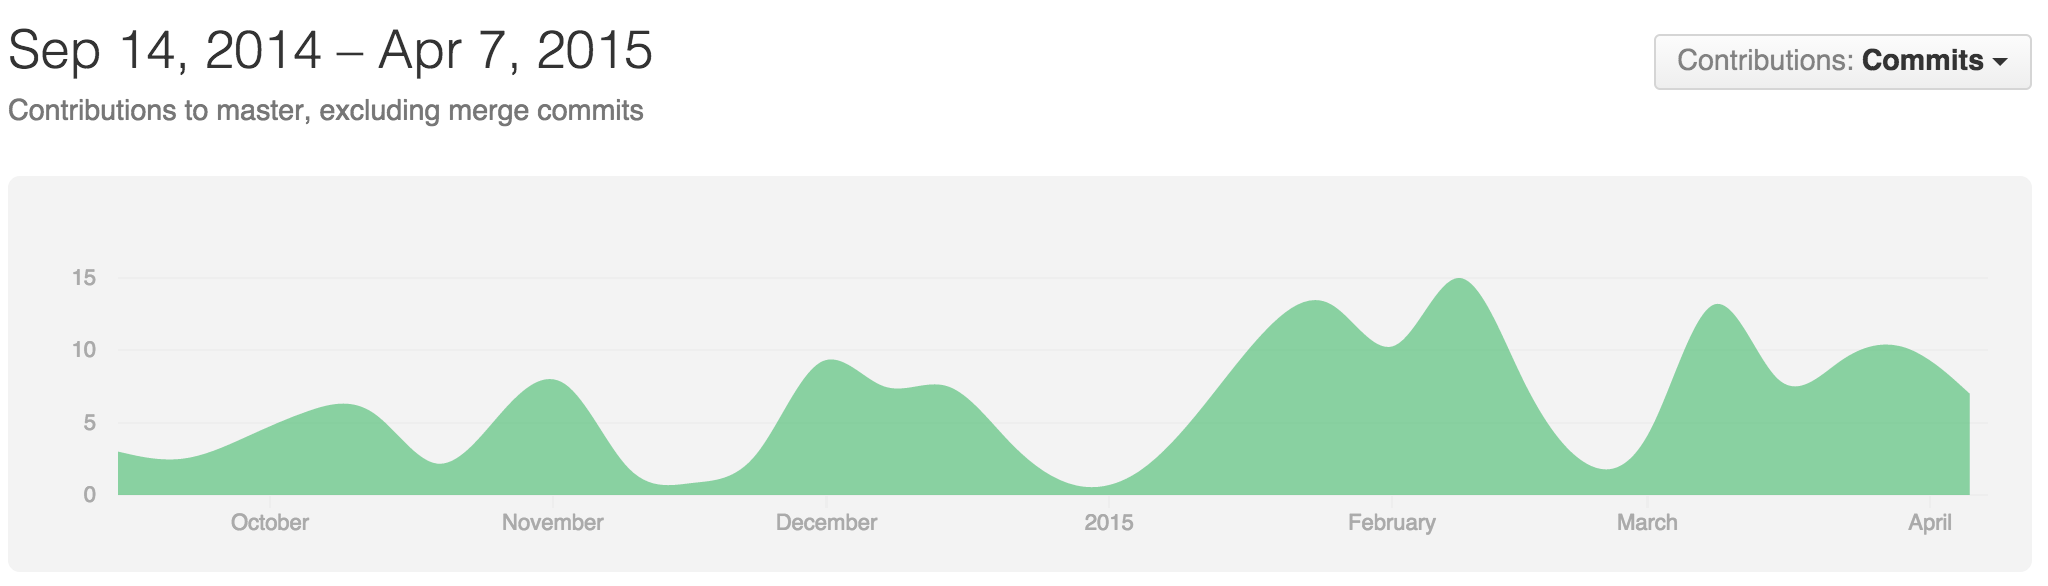
\includegraphics[width=300px]{figures/commit_frequency.png}
  \caption{Commit frequency statistics generated by Github}
\end{figure}
\end{frame}

\begin{frame}{Q\&A}
Thank You!
\end{frame}